%!TEX root = ../report.tex

%%%%%%%%%%%%%%%%%%%%%%%%%%%%%%%%%%%%%%%%%%%%%%%%%%%%%%%%%%%%%%%%%%%%%%%

% \iffalse \fi



\chapter{Arbejdsmarkedets segmentering\label{kapitel_teori_AST}}

%%%%%%%%%%%%%%%%%%%%%%%%%%%%%%%%%%%%%%%%%%%%%%%%%%%%%%%%%%%%%%%%%%%%%%%

% Smid det her ind hvor det passer, måske indledningen, måske et sted i afsnittet, hvem ved, jeg gør ikke haha \#todo
%  Arbejdsmarkedssegmenteringsteorien er det overordnede framework der benyttes i specialet til at forstå arbejdsmarkedets indretning. Centralt i denne står mobiliteten på arbejdsmarkedet samt barrierer for mobiliteten, det vil sige arbejdsmarkedets opdeling i delmarkeder, og hvordan opkomsten af disse delmarkeder skal forstås. Thomas Boje skelner mellem delmarkeder og segmenter, hvor det sidste ses som mere stabile sociale strukturer.

%  Thomas Boje benytter følgende 3 kriterier:

% \begin{itemize}
%   	\item 1. kriterie - Delmarkeder og mobilitet
% 	\item 2. kriterie - Forskellen på et delmarked og et segmenter er forskelle i sociale processeser
%   	\item 3. kriterie - Sociale processer fører til segmentering
% \end{itemize}

% Sociale processer er et meget vagt begreb, hvilket også betyder at segmenter bliver tilsvarende vagt. Ellers bliver det bare empiriske observationer, der viser "klynger af jobtyper med hyppig udveksling." Dette behov for forståelse af de sociale processer der ligger bag segmentering, motiverer følgende: Hvordan kan sociologiens begreber om stratifikation og differentiering bruges til at forstå arbejsmarkedets opdeling i segmenter og delmarkeder? Der findes massere sociologisk teori om stratifikation af mange typer, men fokus vil her være på arbejdsmarkedet og hvad der virker ulighedsskabende på selve arbejdsmarkedet. 



\vspace{20pt} \epigraphfontsize{\small\itshape}
\epigraphfontsize{\small\itshape}
\epigraph{“Labor markets constitute a means of mediation; they reflect the underlying forces in the production and in the laboring population.”}{--- \textup{\parencite[177]{Edwards1979}}}



Denne afhandling tager udgangspunkt i arbejdsmarkedet som \emph{primært} en social struktur, fremfor \emph{primært} et marked, og undersøger om denne sociale struktur udmønter sig i delmarkeder, med forskellige betingelser for lønmodtagerne i dem. Jeg skriver mig ind i traditionen for arbejdsmarkedssegmenterigsteori med dette udgangspunkt.

Denne teoritradition opstod i 1960'ernes USA, og var fremtrædende i 1970'erne og 1980'erne. Teorien er siden blevet taget op igen, i Danmark af bl.a. Toubøl, Larsen og Jensen (\citeyear{Touboel2013}). I korthed går teorien ud på at forstå arbejdsmarkedet som opdelt i segmenter eller delmarkeder, og forklare, hvordan denne opdeling produceres og reproduceres gennem sociale processer.

I dette afsnit vil jeg starte med at beskrive teoriens oprindelige ide om et to-eller tredelt arbejdsmarked, og de fælles kendetegn ved arbejdsmarkedssegmenterigsteorierne.

Derefter vil jeg gå i dybden med Gordon, Edwards og Reichs (GER) tredelte arbejdsmarkedsteori, i deres analyse af det amerikanske arbejdsmarked. GER benytter et framework til at forstå arbejdsmarkedet, jeg mener er nyttigt, og jeg vil udbygge denne med elementer fra Thomas Bojes gennemarbejdning af traditionen, som er specifikt møntet på det danske arbejdsmarked.
GERs segmenteringsteori er blevet undersøgt empirisk igennem de sidste 30 år, og jeg vil gennemgå nogle eksempler,  hvilket giver læseren et godt udgangspunkt for at forstå, hvad status er på empirisk funderet arbejdsmarkedssegmenterigsteori lige nu, og hvad min afhandlings bidrag er i denne forskningstradition. 

Denne afhandling vil tage udgangspunkt i segmenteringsteorierns grundlæggende forståelse af  arbejdsmarkedet og individerne på det, og kun sjældent forholde sig direkte den nyklassisistiske økonomiske skole. For en kritisk empirisk undersøgelse med denne skole i fokus, med udgangspunkt i dennes forståelse af arbejdsløshed, kan man læse Gravholt-Nielsens (\citeyear{Gravholt-Nielsen2016}) specialeafhandling. Det baserer sig på samme datamateriale fra samme årække som denne afhandling. 


%%%%%%%%%%%%%%%%%%%%%%%%%%%%%%%%%%%%%%%%%%%%%%
\section{Den tidlige segmenteringsteori \label{AST_overordnet}}
%%%%%%%%%%%%%%%%%%%%%%%%%%%%%%%%%%%%%%%%%%%%%%

Arbejdsmarkedssegmenteringsteorien opstod historisk som en kritik af og et alternativ til den nyklassisistiske økonomiske skole, hvori arbejdsmarkedet og agenterne på det behandles stort set som et hvilket som helst andet varemarked. Kernen i denne kritik af den nyklassisitiske skole, er en forståelse af individerne på arbejdsmarkedet som drevet, ikke af nyttemaksimerende økonomiske motiver, men bestemt gennem de sociale relationer og institutioner, individerne er indspundet i \parencite[173]{Boje1986}. Jeg vil i det følgende kalde det segmenteringsteori\emph{erne}, da der er tale om teorier med nogle fælles basale antagelser, der dog udmønter sig i vidt forskellige teorier om arbejdsmarkedets funktionsmåder \parencite[177]{Edwards1979}.  Centralt står hypotesen om indkomstfordeling som udtryk \emph{primært} for forskelle mellem delmarkeder, fremfor \emph{primært} som effektiv værdisætning gennem markedsmekanismer på hele arbejdsmarkedet \parencite[78]{BojeToft1989}.

Arbejdsmarkedets funktionsmåde og beskæftigelsespositioner på arbejdsmarkedet er i disse teorier forstået som “\emph{(...) den vigtigste institution, hvorigennem social ulighed og sociale konflikter om fordelingen af samfundets materielle og immaterielle goder opstår og afgøres}” \parencite[10]{Boje1985}. 
% Selvom denne forståelse indenfor sociologien har været kritiseret de sidste femoogtyve år \parencite[23]{Scott2000}, er det udgangspunktet for denne afhandling, at segmenteringsteorien og klasseteorier har ret i denne grundantagelse, om end det anerkendes at betydningen af position på arbejdsmarkedet, særligt i forbrugsvaner og individernes selvforståelse, har ændret sig markant i løbet af det tyvende århundrede. 
% En central forskel fra den neoklassiske skole, er at arbejdsmarkedets heterogenitet og arbejdsstyrkens inhomogenitet er udtryk for grundlæggende sociale strukturer, der fortjener en plads som sådan i teoridannelsen. I den neoklassiske skole antager man markedsmekanismerne som \emph{i princippet} den mest effektive måde at allokere arbejdskraft på arbejsmarkedet, og barrierer for denne allokering skal findes i imperfekt information på markedet, stivhed i løndannelsen på grund af markedsintervenerne instanser såsom fagforeninger (blah blah skriv senere og find henvisning senere. Søren viste mig den der økonomiske grundbog hvor der stod at fagforeninger var en barriere fordi det hindrede den nødvendige frie løndannelse der sikrer effektiv allokering, kan måske bruges \#todo)

Arbejdsmarkedet opfattes i segmenteringsteorierne som bestemt ud fra samfundets struktur og organisering, det vil sige forholdene i produktionen af varer, de institutioner og deres normer, der er opstået som følge af historiske konflikter, samt de forskellige sociale grupper, som arbejdsmarkedet udgøres af \parencite[9]{Boje1985}. Det  vil sige, at disse barierer, som forhindrer principielt fri mobilitet på arbejdsmarkedet, \emph{ikke} ses som barrierer for den fri allokering af arbejdskraft ud fra udbud/efterspørgsmekanismer i et perfekt marked. I stedet ses disse barrierer for mobilitet som grundlæggende sociale mekanismer, som arbejdsmarkedet består af. Arbejdsmarkedet er, som Boje siger, mere kendetegnet af opdeling end af fri konkurrence \parencite[8]{Boje1985}. 

Piorre og Dorringer beskriver lønskelle som udtryk for den amerikanske økonomi opdeling i en kerne- eller primærøkonomi. Kerneøkonomien består af store stabile firmaer, den perifære økonomi består af små, omskiftelige firmaer, med meget usikre markedsvilkår. %\#todo find henvisning
Perioden fra 60'erne og frem til oliekrisen i '73 var en gylden tid for amerikansk økonomi, og der udvikledes en økonomiske struktur, hvor en række af store firmaer nød stabile og gunstige markedsforhold i denne periode. %find henvisning hos dem selv \#todo
Indenfor disse firmaer er arbejdsforholdende relativt gode, og Piorre og Dorringers teori søgte at forklare, hvorfor en stor gruppe mennesker ikke opnåede adgang til de gode jobs i kerneøkonomien. Ambitionen var blandet at at undersøge diskrimination på baggrund af køn og race. Dette blev sat på dagsordenen af borgerrettighedsbevægelsen, kvindefrigørelsen og kvindernes indtog på (dele af) arbejdsmarkedet i perioden \parencites[1216]{Cain1976}. Ideen om en center-perifæri økonomi er inspireret af den amerikanske økonom Robert Averitt (\citeyear{Averitt1968}), der i 1968 skrev en bog med denne tese. Denne opdeling er bundet til en bestemt historisk periode i USAs historie, og det er tvivsomt, hvor meget af denne analyse, der kan overføres til danske forhold. Blandt to åbenlyse forskelle er statens størrelse og den danske erhvervsstruktur, hvor små og mellemstore firmaer fylder langt mere \parencite[36,120]{Boje1985}.  %Blandt andet er den danske virksomhedsstruktur.. hvordan er den? I A&Cs speciale har de en graf, gad vide hvordan det ser ud i Danmark. Kan du se det med registerdata? Eller bare henvis til deres? Du skal ihvertfald vide hvordan den danske virksomhedsstruktur ser ud \#todo.

Det er derfor ikke opdelingen i et primært og et sekundært arbejdsmarked, der skal overføres. Det er måden at gå til arbejdsmarkedet på. Boje opsummerer følgende fællestræk ved segmenteringsteorierne i deres fokus \parencite[106]{BojeToft1989}:  
%
\begin{itemize}
\itemsep-0.7em  
  	\item Diskrimination på arbejdsmarkedet
  	\item institutionelle rammer for arbejdsmarkedet
	\item Interne delarbejdsmarkeder
\end{itemize}
%

En konkret arbejdsmarkedssegmenterigsteori med disse fællestræk samt et fokus på klasseaspektet er Gordon, Edwards \% Reichs teori. Denne er ikke uden svagheder, men har fordel ved at basere sig på (marxistisk) socialklasseteori. Det betyder bindeleddet til de moderne klasseteorier, jeg vil benytte mig af til at forklare forskelle i de sociale processer på delmarkederne, er mere oplagt. Disse klasseteorier har nogle måder at anskue stratifikationen af arbejdsprocesserne på, som jeg mener kan berige arbejdsmarkedssegmenteringsteori. Og omvendt mener jeg GER har en \emph{historisk} og \emph{processuel} anskuelse på arbejdsmarkedets formation og stadige forandring, som jeg finder frugtbar. Dette er - ironisk nok, arven taget i betragtning - noget de moderne klasseforskere har opgivet, til fordel for et fokus på \emph{empirisk operationelle} og \emph{enkle teoretiske} frameworks.


Boje benytter en skillelinje mellem \emph{in-market} og \emph{pre-market} segmentering. Det er forskellen på den stratifikation, der foregår på arbejdsmarkedet, og den, der finder sted før indtrædelsen på arbejdsmarkedet \parencite[46]{Boje1985}. At skelne disse fra hinanden \emph{i praksis} er ikke nemt. Boje opstiller følgende model for forskellen mellem premarket og inmarket segmentering:
%
   \begin{figure}[H]
   \begin{centering}
   	\caption{Premarket og inmarket segmentering}
   	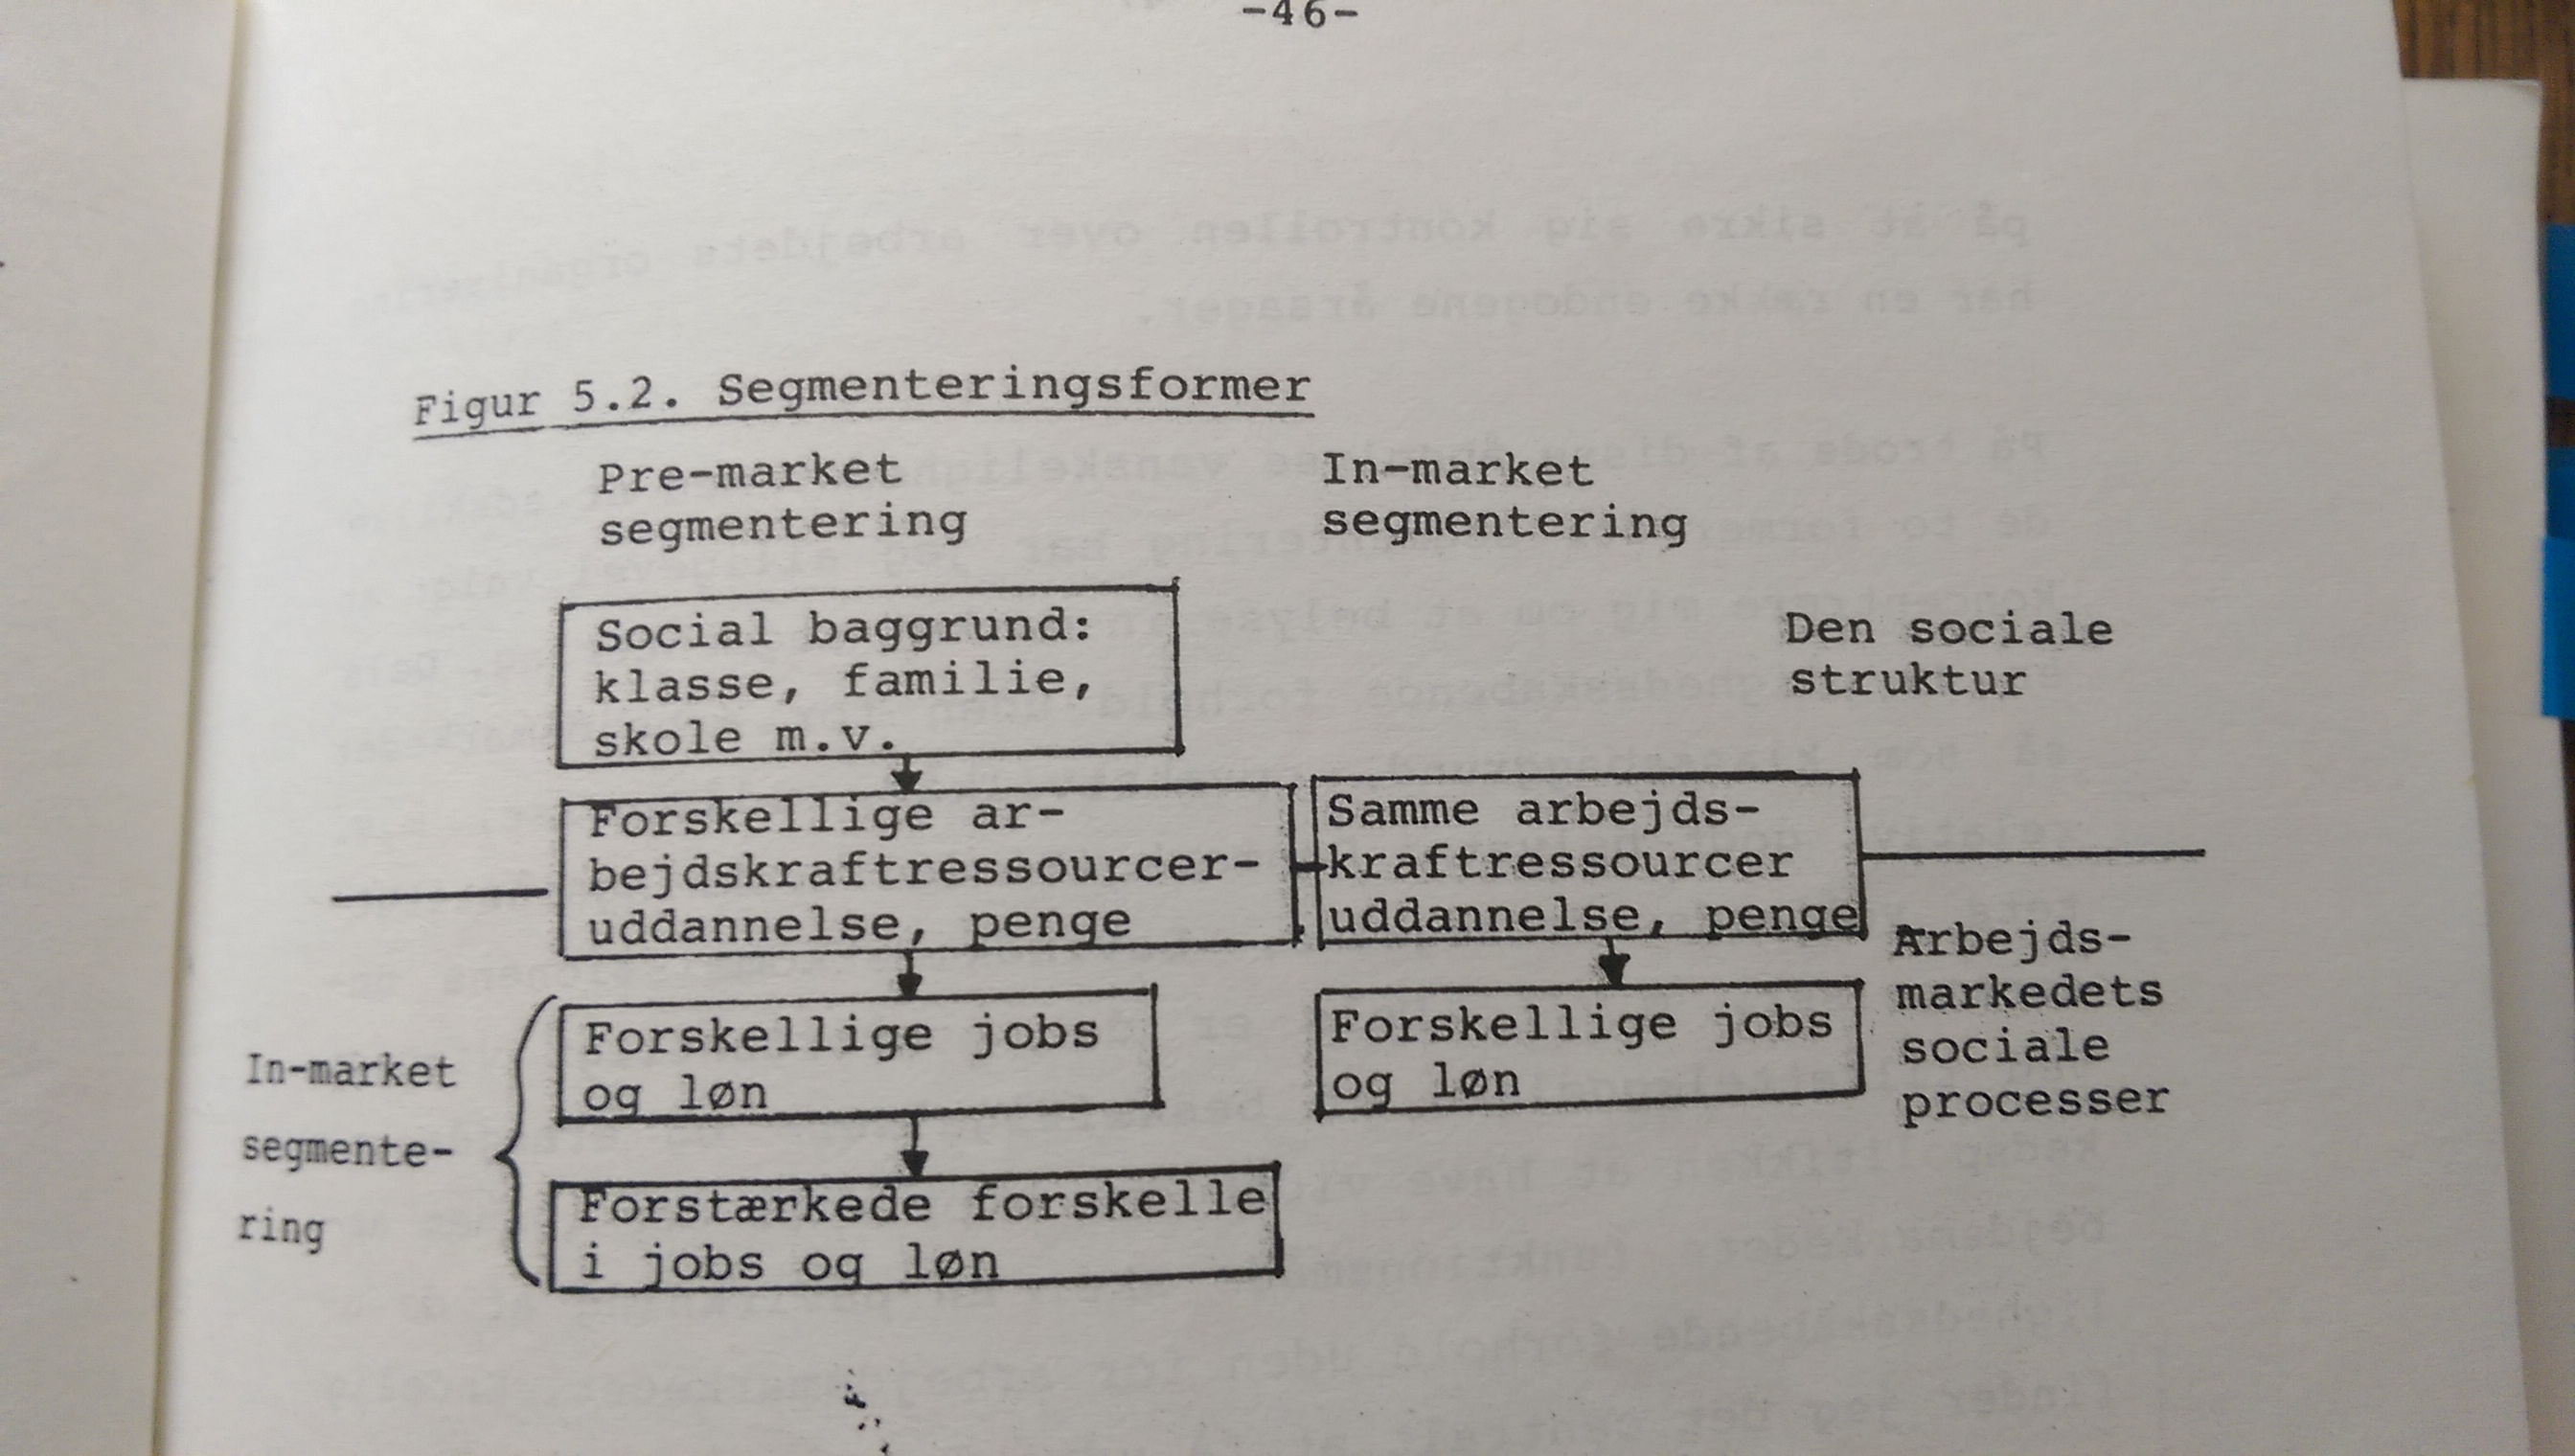
\includegraphics[width=\textwidth]{fig/Boje_premarket_inmarket.jpg}
   	\label{fig_premarketinmarket}
   \end{centering}
   \end{figure}   
%

% \begin{tikzpicture}[>=stealth, thick,font={\tiny}]
% \node (A) at (0,0) [draw, process, text width=2cm, minimum height=0.5cm, align=flush center] 
% {Social baggrund: \\
% klasse,familie, \\
% skole m.v.};

% \node (B) at (3,0) [draw, process, text width=2.5cm, minimum height=0.5cm, align=flush center] 
% {forskellige arb.kraft- \\
% ressourcer: \\
% uddannelse, penge};

% \node (B) at (6,0) [draw, process, text width=2cm, minimum height=0.5cm, align=flush center] 
% {forskellige jobs \\
%  og løn};

% % \coordinate (z) at (0,-3);

% % \draw[->] (A) -- (B);
% % \draw[->] (B) -- (z) -| node[above] {NO} (C);
% % \draw[->] (B) -- (z) -| node[above] {YES} (D);

% \end{tikzpicture}



% \begin{tikzpicture}[>=stealth, thick,font={\tiny}]

% \node (A) at (0,0) [draw, process, text width=5cm, minimum height=0.5cm, align=flush center] 
% {A few lines of text in a block, centered would be nice but not required};

% \node (B) at (0,-2) [draw, double, double distance=1pt, process, minimum height=0.5cm, align=flush center] 
% {A double box here perhaps?};

% \node (C) at (-3,-4) [draw, process, minimum height=0.5cm, align=flush center] 
% {Some words here};

% \node (D) at (3,-4) [draw, process, minimum height=0.5cm, align=flush center] 
% {More words here};

% \coordinate (z) at (0,-3);

% \draw[->] (A) -- (B);
% \draw[->] (B) -- (z) -| node[above] {NO} (C);
% \draw[->] (B) -- (z) -| node[above] {YES} (D);

% \end{tikzpicture}

\emph{Pre-market segmentering } ligger tæt op af hvad man kunne kalde den almene sociale stratifikation i samfundet. Med fokus rettet på de former for stratifikation, der bevirker at lønarbejdere stilles forskelligt ved indtrædelse på arbejdsmarkedet.
Eksempelvis forskelle i kvalitet af uddannelsesinstitutionerne, familiens kulturelle og økonomiske ressourcer, samt  sociale netværk i forbindelse med skolekammerater og familiekontakt, der giver forskellige ressourcer ved indtrædelse på arbejdsmarkedet. 

\emph{In-market segmentering} omhandler de mekanismer, der gør sig gældende på arbejdsmarkedet. Eksempelvis faglig organisering, diskrimination, efterspørgsel efter bestemte færdigheder. Det er denne segmentering, eller \emph{stratifikation}%
%
\footnote{der er meget lidt enighed blandt segmenteringsteoretikere om den præcise definition af segmentering. Selv i den enkelte teoretikers begrebsapparat virker det tilfældigt hvornår segmentering, delmarkeder eller endda stratifikation benyttes. I denne afhandling vil jeg bestræbe mig på at undgå en sådan uklarhed, og kalder det kun pre-market \emph{segmentering} i figur \ref{fig_premarketinmarket}, fordi Boje selv gør det. jeg vil definere min terminologi i slutningen af teori-afsnittet.}%
%
, som GER lægger særlig vægt på i deres segmenteringsteori \parencite[46]{Boje1985}, og i gennemgang af deres teori vil jeg gå i dybdet med dette. 

% påstand om mobilitet på mere end 50 \% men indenfor samme delmarkeder , s. 123 (boje men nielsens bog!!) yes det bekræftiger jeg

Gordon, Edwards og Reichs (GER) benytter opdelingen i et primært og sekundært arbejdsmarked i deres analyse i hovedværket “\emph{Divided Labor, Divided Workers}”, en historisk analyse af det moderne industrielle arbejdsmarkedets opståen og udvikling i USA op til 1970'erne, hvor de mener det segmenterede arbejdsmarked er blevet den dominerende produktionsmåde i landet. GER advarer selv mod at overføre deres middle-range teori direkte til andre lande , i den slags abstrakte teoretisering, som den marxistiske tradition lidt for ofte har haft for vane \parencite[21]{Gordon1982}. Det er derfor mere blikket på arbejdsmarkedet, som jeg mener er nyttigt for at forstå de sociale processer, der skaber arbejdsmarkedets forudsætninger. Vigtig er også GERs egen indrømmelse i slutningen af bogen, hvor de i en diskussion af empirien. De kunne ikke opdele de ikke-manufakturproducerende brancher i deres kerne-perifæri segmenter, da denne distinktion ikke let lader sig overføre udenfor den direkte materielle produktion af goder. I det mindste ikke med den rudimentære data til deres rådighed. Derfor er GERs undersøgelse \emph{en undersøgelse af en tre-delt segmenteringsproces indenfor manufakturen i USA}, \underline{ikke} i hele arbejdsmarkedet. Segmentstrukturen andre steder på arbejdsmarkedet kan være anderledes indrettet, også i USA på det tidspunkt. \parencite[199]{Gordon1982}. Der er derfor al mulig grund til at antage, at en to eller tre-delt segmentstruktur ikke er brugbar i Danmark i informations- og service teknologiernes tidsalder.  Derfor kan elementer af teorien være brugbar til forståelsen af arbejdsmarkeders funktionsmåder generelt, særligt teoriens vægt på de historiske processer, et givent arbejdsmarked på et givent tidspunkt er resultatet af.

%%%%%%%%%%%%%%%%%%%%%%%%%%%%%%%%%%%%%%%%%%%%%%
\section{Edwards, Gordon \& Reich: Det tre-delte arbejdsmarked \label{sec_teori_AST_GER}}
%%%%%%%%%%%%%%%%%%%%%%%%%%%%%%%%%%%%%%%%%%%%%%

 % dårlig start, lav om \#todo
Det spørgsmål, Gordon, Edwards \& Reich stiller - som alle andre marxister efter 2. verdenskrig, kunne man tilføje - er, hvorfor kapitalismens transformering af en bred gruppe af befolkningen til en klasse af arbejdere, ikke endte med en opkomsten af en \emph{klasse-for-sig}, i denne arbejdskraftens homogeniseringsprocess.  De forkaster den traditionelle marxistiske analyse, som “\emph{(...) generate mechanical theories of historical inevitability in which the emergence of a class-conscious proletariat always lurks around the next corner}” \parencite[21]{Gordon1982}. I deres bog \emph{Divided Work, Divided Workers} (1982) benytter de en historisk kontingent analysemetode, inspirereret af bl.a Ernesto Laclau og Eric Olin Wright, der betoner den relative autonomi af politiske og ideologiske kræfter i samfundsudviklingen. GER laver en langsigtet historisk klasseanalyse af hvad de ser som tre perioder i den amerikanske kapitalisme, hvoraf det segmenterede arbejdsmarked er den seneste periode. Selvom analysen en konkret iagtagelse af den historiske udvikling af institutionelle forhold på det amerikanske arbejdsmarked, og amerikanske forhold der spiller ind på dette generelt, er analysemodellen, og dens syn på arbejdsmarkedet, brugbart for denne afhandling, med en række forbehold, der vil blive taget op når det er relevant. 

GER arbejdsmarkedet som et af de vigtigste områder, hvori gennem klassernes sammensætning og relative styrke bestemmes. De skriver:
%
\begin{quote} \small %\raggedright %(bloktekst on/off)
\emph{Here, employers and workers bargain over the effective wage rate, the hours of work, and other elements of the wage-labor contract. The outcome of this bargaining reflects an extraordinarily wide range of forces: the extent to which workers are unified or divided, the intervention of the state, the ability of capitalists to develop new wage-laboring populations, the availability of new labor-saving technologies, the elements of race and ethnicity, the pace of accumulation and hence the strength of the macroeconomy. Nothing the extent of the development of the five major dynamic tendencies of capitalist economies is not sufficient.} \sourceatright{\parencite[21]{Gordon1982}}
\end{quote}
%
Dette skal ses som en vægtning af det de konkrete institutionelle forhold, med særligt fokus på arbejdsmarkedet, som relevant for at forstå økonomien og klassestrukturen i samfundet. I modsætning til en mere abstrakt analyse af de love eller tendenser, der typisk tillægges vægt i en marxistisk-politisk økonomisk analyse, og som GER benævner som de fem store dynamiske tendenser sidst i ovenstående citat: \label{kapitalakkumulation} 1) Kapitalens tendens til at udvide grænserne for det kapitalistiske system, 2) koncentrationen og kontrollen af kapitalen i færre hænder, 3) lønarbejdet udbredes som den dominerende produktionsmåde d4) ændringer af arbejdsprocessen gennem ny teknologi, nye maskiner, nye måder at lede arbejdet på, samt  5) arbejdernes kamp for at beholde eller udvide goder i forbindelse med kapitalens processer. %her kunne godt laves noget fancy med at det den første sætning i hver af de fem punkter blev med fed, eller sådan noget 
Det er GERs argument, at disse fem tendenser i den globale kapitalisme bedst forstås ikke abstrakt teoretisk, men indenfor hvad de kalder \emph{akkumulationens sociale struktur}. Denne sociale struktur defineres som det miljø, hvori det enkelte firma opererer og akkumulerer kapital%
%
\footnote{kapital og akkumulation af denne skal her forstås i marxistisk forstand: Ikke som penge, men som et socialt forhold: \emph{Capital is value in motion}, som David Harvey engang omtalte det som. Den sociale proces, hvori menneskers arbejdstid omsættes til ren bytteværdi, nemlig penge - Hvad Marx kaldte \emph{den universelle ækvivalent} (HENVISNING TIL KAPITALEN), der igen kan investeres i at arbejde, så mere bytteværdi kan udvindes gennem menneskeligt arbejde. Et socialt forhold, således forstået.}%
%
.
Denne gennemgang leder os frem til følgende model i figur \ref{fig_ASSmodel}.
%
\begin{figure}[H]
\begin{centering}
	\caption{ASS-modellen: Model af akkumulationens sociale struktur.}
	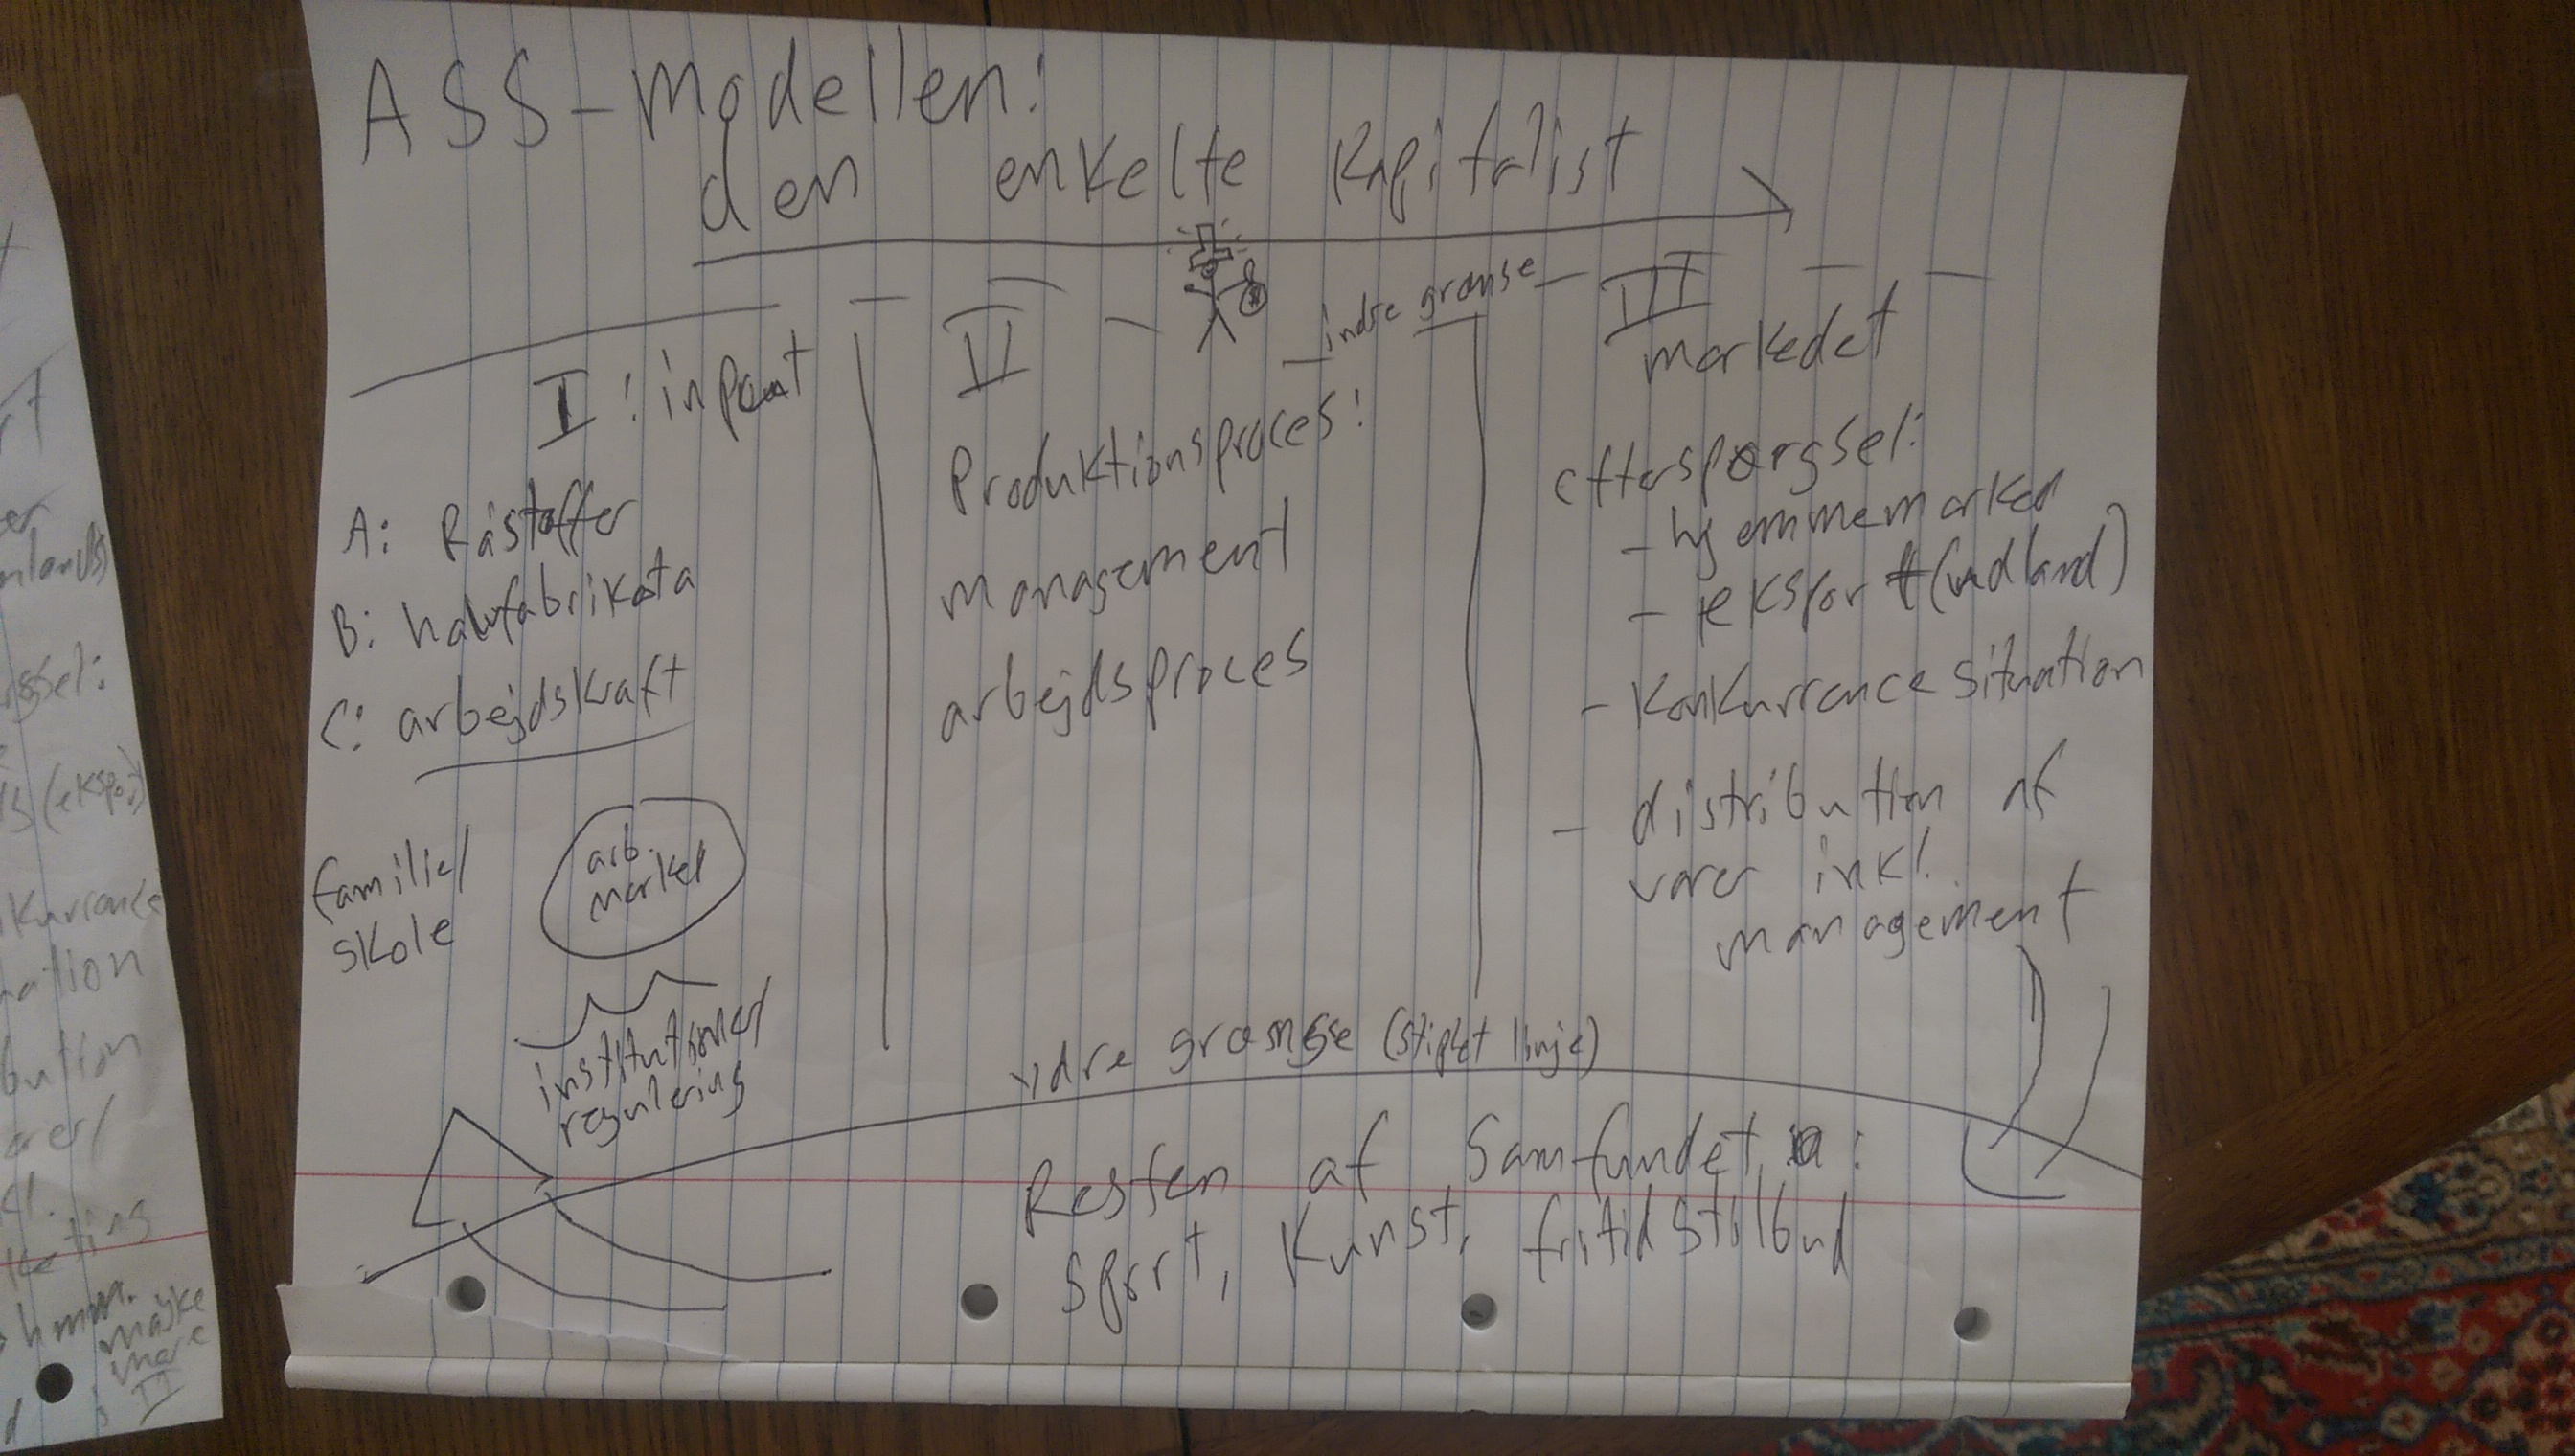
\includegraphics[width=\textwidth]{fig/ASS-model.jpg}
	\label{fig_ASSmodel}
\end{centering}
\end{figure}
%

\emph{I første fase} (I) af kapitalakkumulationen er samlingen af de nødvendige input i produktionsprocessesen. Dette inkluderer råvarer, halvfabrikata og arbejdskraft, hvoraf det sidste nævnes som den mest problematiske af de tre:  
%
\begin{quote} \small %\raggedright %(bloktekst on/off)
Labor supply, the most problematical of the three, involves both structure of the labor market, determining the immediate supply of labor, and the social institutions (family, schools, etc) that reproduce the labor force generationally\sourceatright{\parencite[24]{Gordon1982}} \label{aksocstruk}
\end{quote}
%
Efterspørgslen på arbejdskraft indeholder både arbejdsmarkedet, hvor den nødvendige arbejdskraft med de efterspurgte kompetencer købes på det påkrævne tidspunkt. Det indeholder dog også det langt større felt af sociale institutioner, der sørger for arbejdskraftens sammensætning og kompetenceniveau mere bredt forstået. Det vender jeg tilbage til.

% kunne godt referere til Fligstein her måske

\emph{Anden fase} (II) af kapitalakkumulationen foregår indenfor firmaet selv. Det indeholder organisering af selve arbejdsprocessen og management-strukturen i firmaet. Den fase har ikke så meget med miljøet at gøre som med firmaets interne organisering. GER påpeger at det, der her tilsigtes, er de normer og erfaringer for organisering og management, som firmaerne trækker på, og som derfor er en del af den sociale struktur, det enkelte firma trækker på i dets akkumulationsproces. Denne organisering af arbejdet og ledelsen af arbejdet er central for eksempelvis fagforeningernes betingelser for at organisering. Det har også - lidt mere diffust men ikke mindre vigtigt - vidtrækkende konsekvenser for de livserfaringer, det enkelte menneske gør sig, og dermed hvordan det fortolker verden omkring sig. (REFERENCEMÅSKE? Gruskys kulturelle funktionalisme kunne nævnes her \#todo). 

\emph{Den tredje fase} (III) er salgsprocessen, hvori vareefterspørgsel,  samt status for konkurrencetilstande på det specifikke marked, et givent firma producerer til. Det kunne eksempelvis en være monopollignende tilstand, hvilket muliggør en bestemt virksomhedsstruktur. 

Det er særligt første og anden fase, der har min interesse, da mit fokus er arbejdsmarkedet og dets relation til klassestrukturen. Tredje fase har dog en meget vigtig mekanisme i relation til arbejdsmarkedets segmentering, ifølge GER, som bør fremhæves, og som leder over i GERs teori om det tredelte arbejdsmarked og forklaringen på denne.

Konkurrencetilstanden på markedet har betydning for arbejdsmarkedet generelt, ikke bare af den åbenlyse grund, at det skaber den økonomiske virkelighed for de virksomheder, lønmodtagerne er ansat i. Konkurrencetilstanden på markedet er også en af de væsentligste forudsætninger i GERs segmenteringsteori om et todelt arbejdsmarked. De viser hvordan man I USA fra 30'erne og frem udviklede store firmaer, med stabile profitrater og undertiden monopollignende markedsandele, såvel på hjemmemarkedet som internationalt. Disse firmaers størrelse og stabilitet gav mulighed for \emph{interne arbejdsmarkeder}, hvorigennem kompetencer kan udvikles internt, karrieremuligheder sikrer loyalitet, og andre fordele forbundet med hvad GER kalder \emph{bureaukratisk kontrol}. Dermed menes der management systemer, der strukturerer og sikrer størst mulig samarbejdsvillighed og produktivitet fra arbejderne i arbejdsprocessesen, baseret på nedskrevne love og regler. Det er en af årsagerne til fremkomsten af interne arbejdsmarkeder i store firmaer, der af GER karakteriseres som \emph{kernesegmentet/det primære segment} \parencite[187]{Gordon1982}. Det svært for firmaer fungerende på usikre markeder med lav profitrate at skabe disse strukturer, dette opstår derfor de mest stabile og moderne kapitalisske firmaer, de tenderende-til-monopolitiske, kunne man kan kalde dem.

På denne måde kan vi se at de fem dynamiske tendenser nævnt på \pref{kapitalakkumulation} hænger sammen med den akkumulations sociale struktur, hvorigennem disse lovmæssigheder i en marxistisk optik fungerer. Den femte tendens, arbejdernes modstand, er central for at forstå logikken i segmenteringens opståen, ifølge GER. Det er arbejdernes modtræk, og ikke mindst arbejdsgivernes modtræk til disse modtræk, så at sige. 
Fagforeninger spiller derfor en væsentlig rolle. Det er GERs argument, at fagforeningers styrkeposition fra 30'erne og frem, også i USA, banede vejen for et klassekompromis, hvor arbejdsgiverne blev tvunget til at give indrømmelser omkring stabile ansættelser, reallønstigninger og sikre arbejdsforhold. En række krav blev imødekommet, og arbejdsgiverne var til en vis grad var klar over nødvendigheden af dette. Den tidligere sociale akkumuleringsstruktur, som GER analyserer klassificerer som \emph{homogeniseringsperioden} fra 1870 til slutningen af Anden Verdenskrig, mente man, gavnede radikale elementer i arbejderbevægelsen, da denne skabte homogenitet i klassestrukturen blandt arbejderklassens forskellige fraktioner. Derfor var visse indrømmelser at foretrække. Der var desuden nok at gøre med at tilrettelægge arbejdsprocessen til ny teknologi og nye måder at styre, uddanne og inddele arbejdsstyrken på. Her kunne fagforeninger også bruges som nødvendige samarbejdspartnere \parencite[186f]{Gordon1982}. Denne overgivelse af magt over arbejdsprocessen, som fagforeninger gav - eller blev tvunget til - attribuerer GER til tre hovedårsager, nemlig muligheden for reallønstigninger og sikringer af arbejdstagerrettigheder. Det  muliggjordes af det økonomiske boom efter 2. Verdenskrig. De to andre faktorer var udrensning af radikale elementer i fagforeningerne i McCarthy-æraen, samt den manglende evne til at forstå hvad denne overgivelse af magt til arbejdsgiverne i arbejdsprocessen betød for lønmodtagernes styrkeposition. Dette danner basis for en primærøkonomi og en perifær økonomi, der skal gennemgås nu.

%%%%%%%%%%%%%%%%%%%%%%%%%%%%%%%%%%%%%%%%%%%%%%
\section{De to primære segmenter og det sekundære segment \label{AST_primuafprimundersekundaer}}
%%%%%%%%%%%%%%%%%%%%%%%%%%%%%%%%%%%%%%%%%%%%%%


Logikken i det nye system, der derved blev udviklet, kan opsummeres på følgende vis: Jobs blev findelt i specifikke jobfunktioner, ofte indenfor trin i en karriertrappe. Ny teknologi påvirkede ikke kun hastigheden og arbejdskvaliteten, men blev også benyttet med det bredere formål at akkomodere managementpolitik, reguleringen af arbejdet og arbejderne som sådan. Ansættelser, forfremmelser og afskedigelser blev systematiseret og bureaukratiseret. Forhandlinger mellem arbejdergiver-fagforeninger blev i højere grad et spørgsmål om løn og frynsegoder, mens arbejdsforholdene og arbejdspladsens indretning blev til managementpolitik, udviklet af ingeniører og forløberne til HR-konsulenter. Det betyder at arbejdsmanagement skiftede karakter fra en intervention fra ledere eller mellemledere og deres direkte autoritet, til et spørgsmål om regulativer og procedurer \parencite[189]{Gordon1982}%
%
\footnote{Udviklingen af bureaukratisk autoritet er en tendens Max Weber beskriver så tidligt som i 20'erne. Jeg anskuer det sådan, at GER viser hvorledes denne autoritetsform rodfæster sig i den samfundsmæssige produktion i årtierne efter, og at dens konkrete udformning og formål - udover at have sin egen indre logik, jvf. “rationalitetens jernbur” - sker på basis af magtkampe mellem klasserne. (FIND HENVISNING WEBER).}%
%
. 

Det betyder dog ikke, at alle arbejdstagere i den primære økonomi har samme forhold. GERs såkaldt todelte arbejdsmarkedsteori er mere en teori om et \emph{tredelt} arbejdsmarked. Deres fokus på \emph{firmaer} som central økononomisk enhed, samt den i forvejen etablerede forskning om center-periferien i amerikansk økonomi, får dem til at tale om det primære og sekundære segment, fordi det er sådan, det findes på firma-niveau. Hvis man kigger på beskæftigelsesforhold, viser GERs analyse imidlertidig en opdeling af arbejdet i primærfirmaer i to segmenter: Det \emph{“primære uafhængige”} segment og det “\emph{primære underordnede}” segment. Disse segmenter fungerer i store firmaer med de tidligere nævnte karakteristikker, og begge segmenter har, relativt til det sekundære segment, højere lønninger, bedre jobsikkerhed og mulighed for karriereveje \parencite[202]{Gordon1982} \label{GERs tre segmenter}. Det er denne virksomhedsstruktur, der danner basis for det primære segment af arbejdstagere.

Det \emph{sekundære/perifære} segment består af job i små og mellemstore virksomheder, ofte ejet af et enkelt individ eller en familie, i begrænsede markedspositioner, tit med usikker eller stærkt variende efterspørgsmål. Profitten er typisk lavere end i kerneøkonomien
, og økonomiske kriser resulterer ofte i konkurs eller alvorlige finansielle problemer. Teknologi og marketing er sjældent up to date med firmaer i kerneøkonomien \parencite[7]{Averitt1968}. Det sekundære arbejdsmarked har som følge deraf lavere lønninger, større risiko for arbejdsløshed, mange midlertidige  stillinger og andre dårlige ansættelsesforhold \parencite[70f]{Doeringer1971}.

GER peger på at firmaer i den perifære økonomi tjener et formål, og der er grunde til at de ikke overtages af kernefirmaerne: Det er usikre markeder med svingende, ofte lavt, afkast. Det giver kernefirmaer mulighed for outsourcing af bestemte opgaver, der er billigere end indenfor de restriktioner, det primære beskæftigelsessegment muliggør. Særligt i forbindelse med varierende efterspørgsel: Det giver en fleksibilitet i at kunne hyre arbejdere fra det sekundære segment indirekte, gennem et sekundært firma, når efterspørgslen på et primærfirmas varer er høj, uden at være bundet op på forpligtigelser når efterspørgslen er lav \parencite[191]{Gordon1982}. 

Det primære uafhængige segment \label{GER kontrol og intern arb marked} indeholder de højere uddannede lønmodtagere indenfor professionerne, management og teknisk arbejde. De oplever et højere økonomisk afkast ved deres uddannelse%
% 
% \footnote{GER skriver at de opnår “\emph{a higher return to schooling and experience}” \parencite[202]{Gordon1982}, hvilket jeg tolker som \emph{relativt} til det underordnede segment, det vil sige at de økonomisk får mere ud af x antal års uddannelse eller erfaring end en person beskæftiget i det underordnede segment.}% ligegyldig fodnote er det ikke? \#todo
%
, og der er sjældent en direkte supervision af og autoritetsudøvelse over udførslen af deres arbejde. De er desuden tilbøjelige til at internalisere firmaets formål. 
Historisk udspringer dette, ifølge GER, af proletariseringen og de deraf følgende konsekvenser af nogle traditionelle klasser i forbindelse med kapitalismens tidligere akkummulationsstruktur, i GERs jargon kaldet \emph{homogeniseringsperioden}.  Dette skete indenfor eksempelvis håndværkerlaug, samt andre med højtudviklede faglige ekspertiser. Ekspertise på de niveauer var i midlertidigt en nødvendighed, og en omkalfatring af disse traditionelle klasser ledte til fremkomsten af positioner i den primære økonomi, hvoraf formel uddannelse med tæt tilknytning til “arbejdsmarkedets behov”, altså arbejdsgivernes behov, fandt sted. Det skete  ifølge GER ikke uden magtkampe mellem klasserne, så GER pointerer at disse erhvervsgruppers nuværende position også er et resultat af de modtræk, erhvervsgrupperne benyttede sig af, for at sikre sig autonomi og andre goder, eksempelvis ved oprettelsen af hvad GER kalder “professionelle associationer”, man kunne forestille sig at DJØF og IDA kunne eksempler i en dansk kontekst. Resultatet af denne torvtrækning med arbejdsgiverne, til en vis grad vellykket, betød følgelig skarpere segmentering ifht. det primære underordnede segment \parencite[202f]{Gordon1982}.

Det \emph{sekundære/perifære} segment består af job i små og mellemstore virksomheder, ofte ejet af et enkelt individ eller en familie, i begrænsede markedspositioner, tit med usikker eller stærkt variende efterspørgsmål. Profitten er typisk lavere end i kerneøkonomien
, og økonomiske kriser resulterer ofte i konkurs eller alvorlige finansielle problemer. Teknologi og marketing er sjældent up to date med firmaer i kerneøkonomien \parencite[7]{Averitt1968}. Det sekundære arbejdsmarked har som følge deraf lavere lønninger, større risiko for arbejdsløshed, mange midlertidige  stillinger og andre dårlige ansættelsesforhold \parencite[70f]{Doeringer1971}.

GER peger på at firmaer i den perifære økonomi tjener et formål, og der er grunde til at de ikke overtages af kernefirmaerne: Det er usikre markeder med svingende, ofte lavt, afkast. Det giver kernefirmaer mulighed for outsourcing af bestemte opgaver, der er billigere end indenfor de restriktioner, det primære beskæftigelsessegment muliggør. Særligt i forbindelse med varierende efterspørgsel: Det giver en fleksibilitet i at kunne hyre arbejdere fra det sekundære segment indirekte, gennem et sekundært firma, når efterspørgslen på et primærfirmas varer er høj, uden at være bundet op på forpligtigelser når efterspørgslen er lav \parencite[191]{Gordon1982}. 

Det primære uafhængige segment \label{GER kontrol og intern arb marked} indeholder de højere uddannede lønmodtagere indenfor professionerne, management og teknisk arbejde. De oplever et højere økonomisk afkast ved deres uddannelse%
% 
\footnote{GER skriver at de opnår “\emph{a higher return to schooling and experience}” \parencite[202]{Gordon1982}, hvilket jeg tolker som \emph{relativt} til det underordnede segment, det vil sige at de økonomisk får mere ud af x antal års uddannelse eller erfaring end en person beskæftiget i det underordnede segment.}%
%
end de to andre segmenter, og der er sjældent en direkte supervision og autoritetsudøvelse forbundet med udførslen af deres arbejde. De er tilbøjelige til at internalisere firmaets formål som deres egne.
Historisk udspringer dette, ifølge GER, af proletariseringen og de deraf følgende konsekvenser af nogle traditionelle klasser i forbindelse med kapitalismens tidligere akkummulationsstruktur, i GERs jargon kaldet \emph{homogeniseringsperioden}.  Dette skete indenfor eksempelvis håndværkerlaug, samt andre med højtudviklede faglige ekspertiser. Ekspertise på de niveauer var i midlertidigt en nødvendighed, og en omkalfatring af disse traditionelle klasser ledte til fremkomsten af positioner i den primære økonomi, hvoraf formel uddannelse med tæt tilknytning til “arbejdsmarkedets behov”, altså arbejdsgivernes behov, fandt sted. Det skete naturligvis ikke uden klassekamp, så GER pointerer at disse erhvervsgruppers nuværende position også er et resultat af de modtræk, erhvervsgrupperne benyttede sig af, for at sikre sig autonomi og andre goder, eksempelvis ved oprettelsen af hvad GER kalder “professionelle associationer”, man kunne forestille sig at DJØF og IDA kunne eksempler i en dansk kontekst. Resultatet af denne torvtrækning med arbejdsgiverne, til en vis grad vellykket, betød følgelig skarpere segmentering ifht. det primære underordnede segment \parencite[202f]{Gordon1982}.
Dette kan også tolkes som GERs bud på hvad Eric Olin Wright kalder “the problem of the middle classes” i marxismen, altså hvilken historisk rolle og nuværende position, man skal forstå middelklasserne i, i en marxistisk optik. Mere om det i afsnit (??? \#todo).

Det “\emph{primære underlagte}” segment har ikke nødvendigvis udsigt til betydningsfulde forfremmelser, men er i stedet motiveret af stabil jobsituation og lønforhøjelser gennem anciennitet. Deres arbejdsprocess er superviseret og indeholder meget repetitivt, rutinepræget arbejde, med specifikke regler for dets udførsel og direkte autoritetsudøvelse i forbindelse med overholdelsen af disse. Der er ikke kun tale manuelt arbejde af den traditionelle arbejderklasse-forestilling, men også ikke-manuelt arbejde indenfor “\emph{white-collar}”jobs befinder sig i det primære underordnede segment (du må ku finde på en bedre beskrivelse \#todo) .  Disse er i langt højere grad organiseret sig gennem fagforeninger, da loyalitet til arbejdsgiverne ligger fjernere for beskæftigede i dette segment end i det primære uafhængige segment. \parencite[28f]{Drago1995} og \parencite[203]{Gordon1982}. (hvordan kan jeg få de her stå i samme parentes? \#todo). tolkes som GERs bud på hvad Eric Olin Wright kalder “the problem of the middle classes” i marxistisk klasseteori: Hvilken historisk rolle og nuværende position kan man forstå fremkomsten af en lang række klassefraktioner, der ikke så let kan karakteriseres som arbejderklasse. Mere om det i afsnit (??? \#todo).

Det “\emph{primære underlagte}” segment har ikke nødvendigvis udsigt til betydningsfulde forfremmelser, men er i stedet motiveret af stabil jobsituation og lønforhøjelser gennem anciennitet. Deres arbejdsprocess er superviseret og indeholder meget repetitivt, rutinepræget arbejde, med specifikke regler for dets udførsel og direkte autoritetsudøvelse i forbindelse med overholdelsen af disse. Der er ikke kun tale manuelt arbejde af den traditionelle arbejderklasse-forestilling, men også ikke-manuelt arbejde indenfor “\emph{white-collar}”jobs befinder sig i det primære underordnede segment (du må ku finde på en bedre beskrivelse \#todo) .  Disse er i langt højere grad organiseret sig gennem fagforeninger, da loyalitet til arbejdsgiverne ligger fjernere for beskæftigede i dette segment end i det primære uafhængige segment. \parencite[28f]{Drago1995} og \parencite[203]{Gordon1982}. (hvordan kan jeg få de her stå i samme parentes? \#todo).

GERs historiske redegørelse for klasseudviklingen i USA er, naturligvis, netop dette: en redegørelse for klasseudviklingen \emph{i USA}. Det betyder at en lang række af de sociale forhold, der gør sig gældende, ikke kan overføres til andre lande. Sammensætningen og betydningen af hvilke sociale strata, der findes, hvordan middelklassepositionerne er udformet, samt hvilke politiske alliancer, der findes. Det er centralt for udformingen af et samfund, som de siger, og fortsætter: “\emph{an emphasis on human agency rather than abstract laws in historical change, (...) the importance of historical contingency in shaping the responses of different groups to capitalist development, (...) and the diverse spatial and temporal paths of capitalist development.}” \parencite[21]{Gordon1982}. 

Det er derfor tankegangen og forståelsen af, hvorledes arbejdsmarkedet fungerer i klassestrukturen, der er brugbar i min afhandling. Denne vil jeg benytte i min egen analyse. 
Det kan være svært at lave en præcis grænse mellem disse to typer segmenter. I en dansk kontekst konkluderer Andrade, i en registerdata-baseret undersøgelse af nabolagseffekter på indkomstforskelle i perioden 1986-1988 og 2006-2008: “\emph{Although changes in the labour market appear to be the primary factor in the explanation of the reproduction of poor and wealthy neighborhoods, geographical movements can be viewed as a spill-over-effect in which individuals who no longer fit the socioeconomic profile of the neighborhood moves out of the the neighborhoods. These selection processses of geographical mobility in and out of neighborhoods have an active role in changing the neighborhood enviroment.}” \parencite[134]{Andrade2014}. Det vil sige, at selv det (kultur)geografiske landskab er påvirket af arbejdsmarkedets sammensætning - arbejdsmarkedet påvirker premarket segmenteringen, her forstået som geografiske fordelinger af forskellige arbejdstagere i landet. Denne socioøkonomiske fordeling, der hører ind under premarket segmentering, virker tilbage pp mulighederne på arbejdsmarkedet, altså inmarket segmenteringen. Hvad, som man siger, kom først: Hønen eller ægget? Hvor svaret naturligvis er, at det er det forkerte spørgsmål at stille i den sammenhæng, fordi der ikke er en \emph{sui genesis} kausalitet på spil. Det gælder denne kulturgeografiske - klassemæssige sammenhæng, såvel som den gælder opdelingen mellem inmarket - og premarket segmentering. 

Derfor kan det naturligvis \emph{analytisk} give mening at lave et klart skel mellem sociale processer, der foregår direkte på arbejdsmarkedet, og de processer, der er en del af hele klassestrukturen. Det er inkorporeret i følgende udvikling af ASS-modellen, nu kaldet B-ASS (for Boje): 
%
\begin{figure}[H]
\begin{centering}
	\caption{B-ASS modellen}
	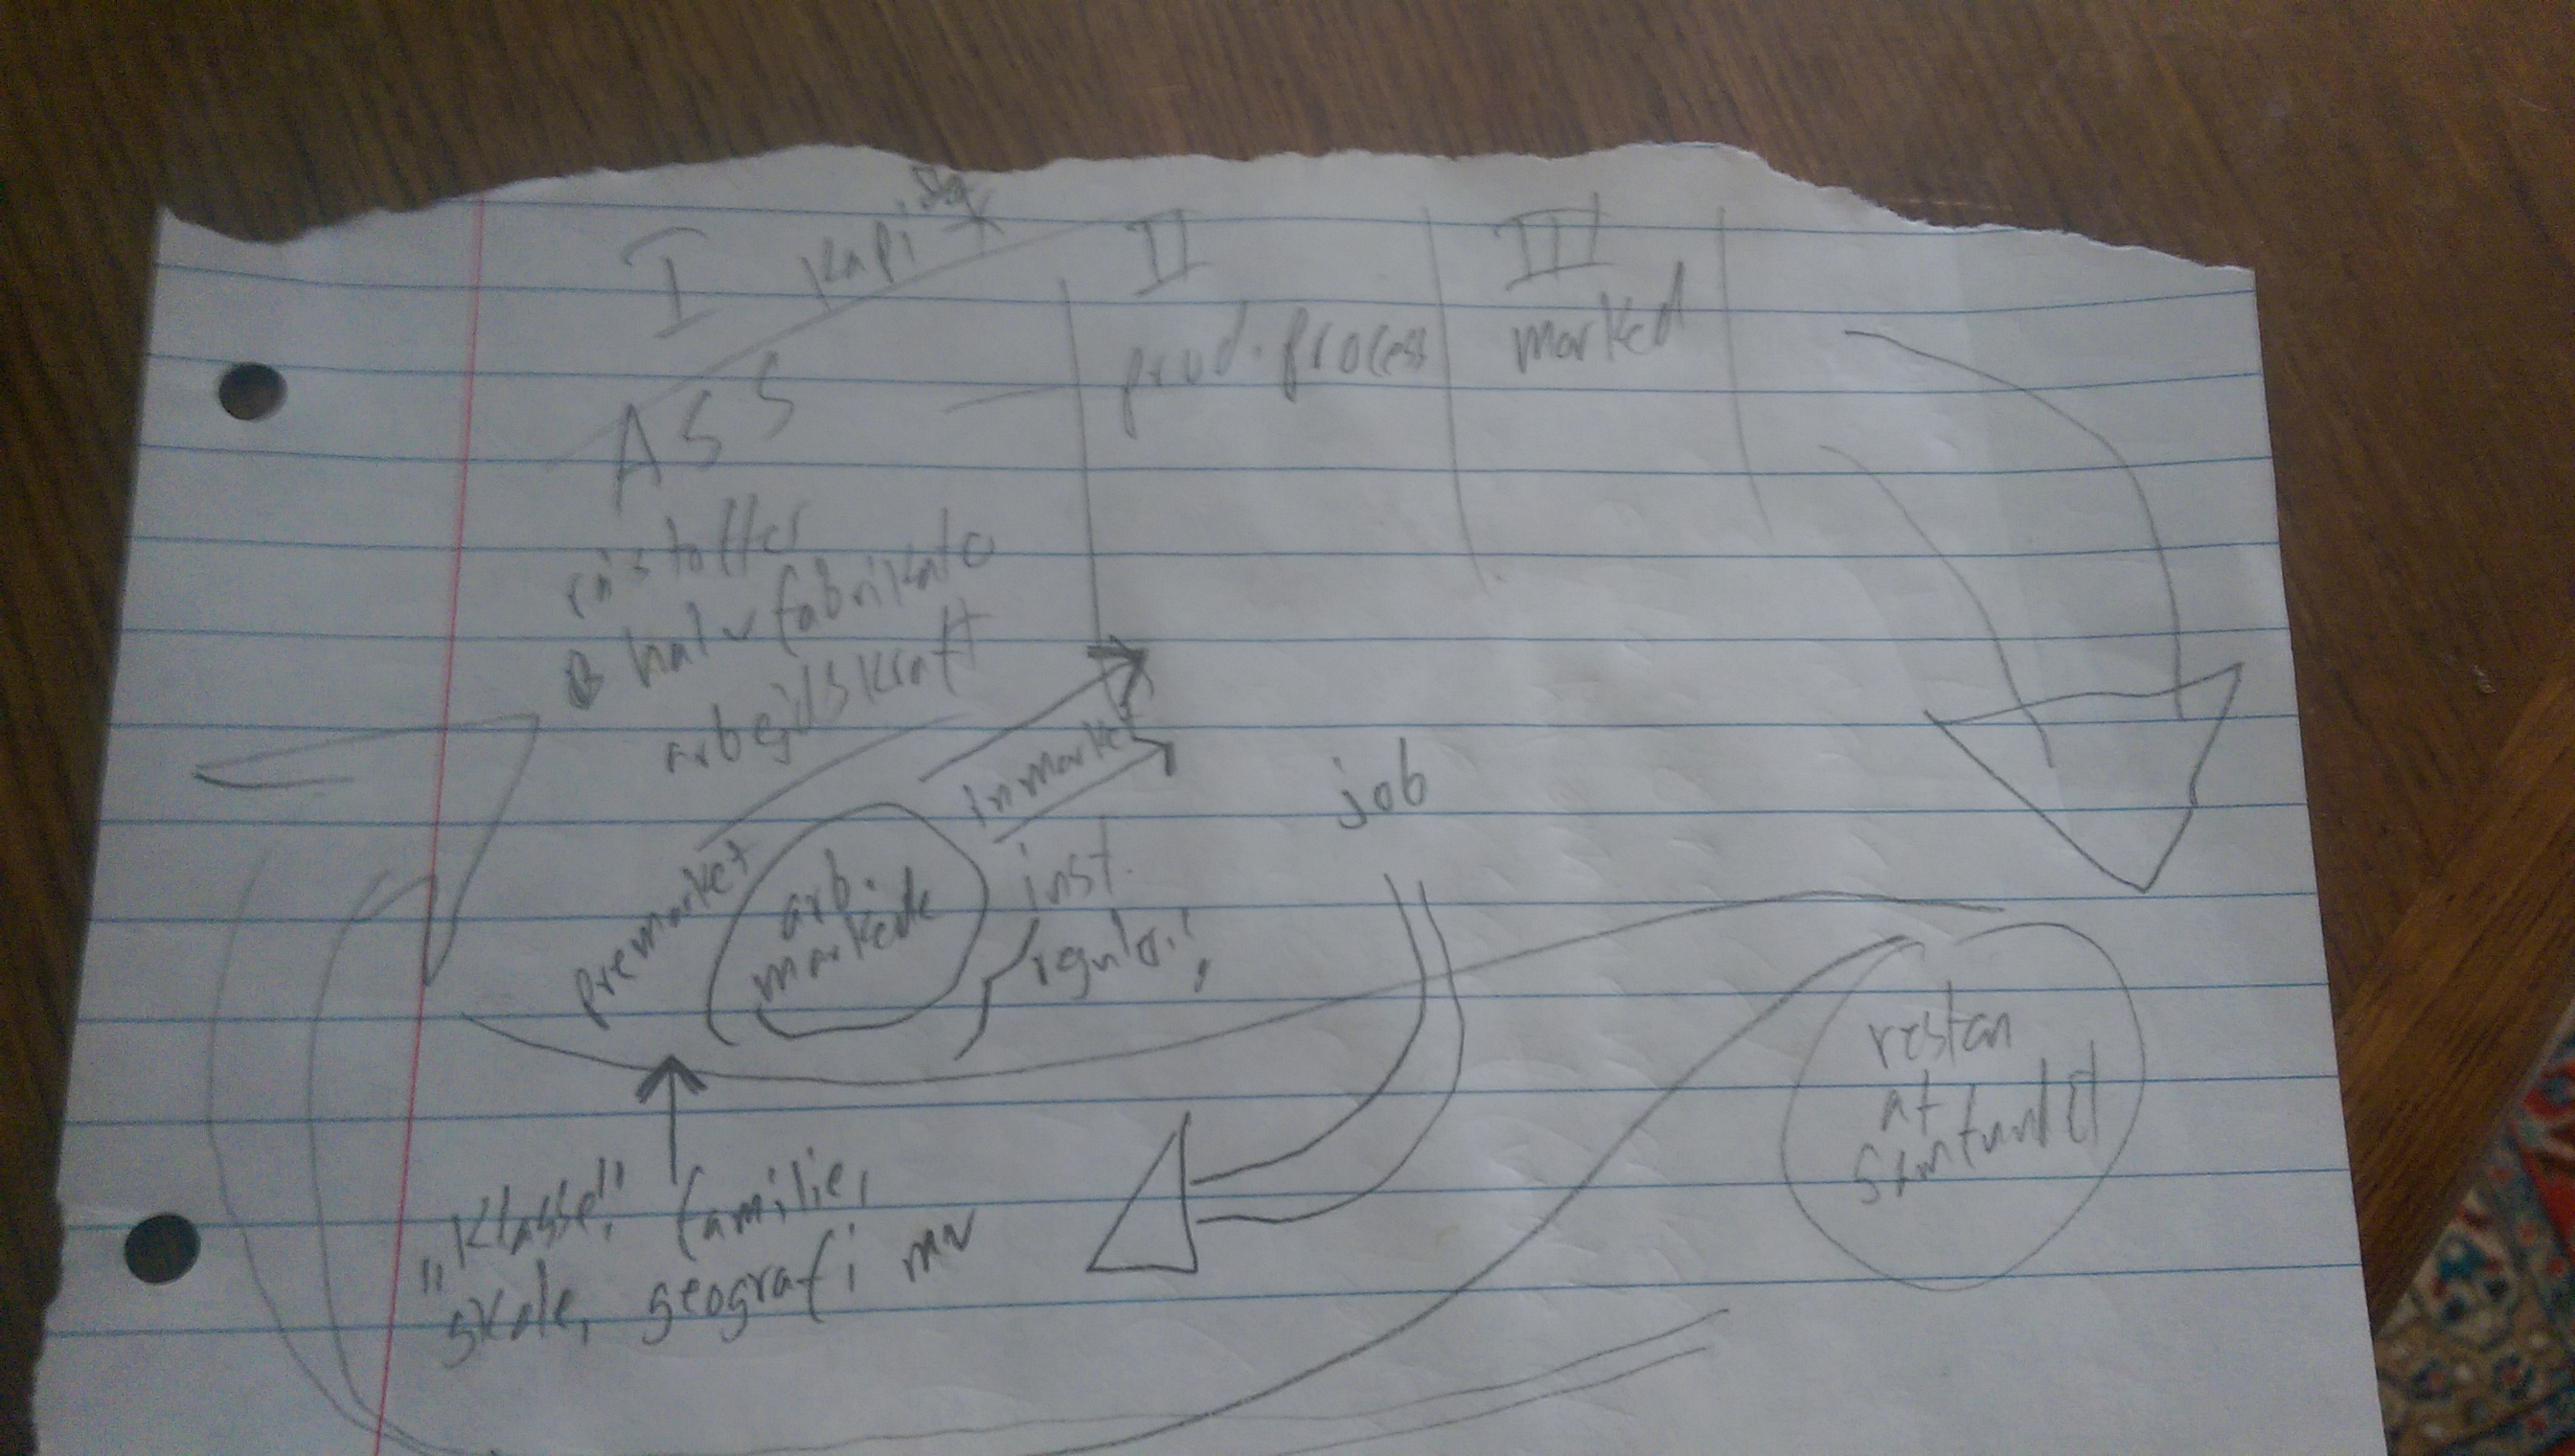
\includegraphics[width=\textwidth]{fig/B-ASS-model.jpg}
	\label{fig_B-ASSmodel}
\end{centering}
\end{figure}
%

mangler ordentlig gennemgang af B-ASS modellen \#todo.


%%%%%%%%%%%%%%%%%%%%%%%%%%%%%%%%%%%%%%%%%%%%%%
\section{Empiriske resultater og metodologiske udfordringer  \label{sec_teori_AST_metodeogempiri}}
%%%%%%%%%%%%%%%%%%%%%%%%%%%%%%%%%%%%%%%%%%%%%%


Skriv bedre indledning \#todo

Derudover har GERs teori samt empiri nogle problemer, der skal adresseres. Først de empiriske udfordringer samt bud på kortlægninger af segmenter, jeg har set på.

Det er en alvorlig udfordring i segmenteringsteori, at der er meget lidt enighed om hvad der præcist karakteriserer et segment, hvordan segmenter er adskilt fra hinanden, og følgelig hvordan man empirisk observerer segmenter \parencite[71]{Leontaridi1998}, \parencite[1231]{Cain1976}. Følgelig er de indikatorerer og variable, der benyttes til at observere segmenter, vidt forskellige. Jeg vil her beskrive tre strategier, som jeg ser i litteraturen. Disse tre strategier benytter sig af forskellige variable, samt forskellige statistiske teknikker. 

Gordon, Edwards og Reich er overraskende vage i deres empiriske definition af hvad der udgør et segment, og hvordan det bør måles.
De benytter selv data på branche-niveau, men siger at brancher  indeholder både kerne- og perifæri firmaer. De mener med andre ord at data på firmaniveau er ideelt, men har ikke sådanne data til rådighed selv \parencite[193]{Gordon1982}. De indikatorer, de benytter sig af, er primært mål for økonomisk formåen på brancheniveau, hvori beviset for den 3-delte segmentering, de a priori har inddelt brancherne i, handler om den relative forskel mellem segmenterne på en række indikatorer, og særligt en stigende relativ forskel over tid. 
Det er indikatorer såsom værdi tilført per arbejder, lønforskelle per arbejder, andelen af manuelt arbejdende i forhold til ikke-manuelt arbejdende i firmaet, samt faglig organisering i branchen. Alle disse sættes op relativt mellem GERs på forhånd inddelte 3-delte segmentopldeing \parencite[193]{Gordon1982}. 

Derudover kommer de med to interessante betragtninger om ting de \emph{ikke} har kunne måle: Udover at de helst ville have data på firma-niveauer, siger de også at indenfor firmaer i den primære økonomi, findes der sekundære og primære jobtyper. Derfor ville data på beskæftigelsesniveau fremfor firma- og branche være interessant\parencite[193]{Gordon1982}. 



Man kan sammenfatte og sige at denne metode inddeler brancher efter en teoretisk styret logik baseret på et tre-delt arbejdsmarked, og benytter økonomiske nøgletal på brancheniveau som variable. Nøgletallene er antageligt populationsbaserede, fremfor survey-baseret (bliv sikker på det her senere \#todo) Herefter benyttes forskellene i nøgletallene mellem de tre teoretisk inddelte segmenter til at teste hypoteser om forskelle på segmenterne. De benyttede variable har et fokus på produktion og fagforeningsorganisering til at lave denne tredeling. At analyseenheden dermed bliver brancher, har været under skarp kritik grundet sin overordnede og upræcise natur (boje 1988: 84)


Den anden strategi er benyttet i en australsk undersøgelse fra 1995, hvor Robert Drago (1995) finder at den tredelte segmentstruktur beskrevet af GER passer med det australske arbejdsmarked. Her benyttes survey-data på firma-niveau, og metoden er en  konfirmatorisk klusteranalyse. Det vil sige antallet af klustre er bestemt ex ante til GERs tre segmenter. At observationsenheden er firmaer, giver nogle problemer, bemærker Drago selv, da firmaer godt kan indeholde job fra forskellige segmenter, men denne undersøgelse gør det til enten-eller. Variablene er andelen af manuelt arbejdende i forhold til ikke-manuelt arbejdende i firmaet, andelen af ansatte med jobancienittet på mindst 10 år, andelen af deltidsansatte, andelen af kvindelige ansatte, lønningsniveauer, andelen af supervisorer der er steget i graderne internt i firmaet og deslige. Drago finder at de tre klustres karakteristikker passer overordentligt godt med den tredelte segmentstruktur i GERs segmenteringsteori \parencite[59]{Drago1995}. 

Man kan sige sammenfatte og sige at her er den empiriske metode ganske avanceret, og baseret en survey hvor observationsenheden er firmaer, som anbefalet af GER selv. Segmentinddelingen af firmaerne er ikke lavet af forskerne selv, men af en konfirmatorisk klusteranalyse, der baserer sine grupperinger på minimal varians af variable indenfor det på forhånd fastsatte antal klustre. Selve variablene er mindre fokuseret på økonomisk formåen i segmenterne og mere fokuseret på arbejdsmiljø. 

Gittleman og Howell (1995) benytter ligeles klusteranalyse deres undersøgelse af segmenter, men ud fra et andet udgangspunkt. De opsummerer segmenteringsteoretikernes empiriske forsøg på følgende vis: “\emph{the most common approach in empirical studies of segmentation, particularly when the unit of analysis is occupations, has been to begin with the researcher's judgment about how many and what kind of rules to empirically implement the scheme, again based on the researcher's judgment. (...) the arbitrariness of this approach has been sharply critized.}” \parencite[422]{Gittleman1995}. Derfor benytter de i stedet en eksplorativ klusteranalyse, hvor antallet af segmenter ikke er defineret på forhånd. De benytter Wards hierarkisk-agglomerative klusterteknik. Det betyder at klustre merges sammen på stadig højere niveauer, sådan at to klustre, der merges på 2. niveau af klusterproceduren, hver især godt kan være sammenlægninger af tidligere klustre på 1. niveau, og så fremdeles, indtil visse varians-kriterier er opfyldt \parencite[425]{Gittleman1995}.
Man kunne måske forledes til at tro at de mener en udelukkende mekanisk inddeling er at foretrække, det er dog for simpelt. De når frem til 6 klustre, hvor de udelader en 7. kluster af teoretisk-praktiske grunde - de argumenterer for denne 7. gruppe er en undergruppe af et af de andre segmenter, da de sammenlagte jobtyper ikke adskiler sig væsentligt \emph{på et teoretisk niveau indenfor segmenteringsframeworket} fra den klynge, den kommer fra \parencite[424]{Gittleman1995}. Så der er mere tale om at beslutte sig for en deskriptiv statistisk teknik, hvorigennem ligheder og forskelle defineres ud fra, og et bud på en segmenteringsstruktur foreligger. Og derefter fortolke denne struktur teoretisk, finde ud af hvor den simpelthen ikke giver mening, fordi den udelukkende er teknisk fremstillet, og modificere de tekniske parametre, der ligger til grund, således at en meningsfuld model kan benyttes. Altså en abduktiv empirisk tilgang (find reference på abduktiv \#todo). Men grundlæggende 

De benyttede variable kommer fra en survey om arbejdskvalitet, og detaljerede informationer om respondernes beskæftigelse samt branche-tilhørsforhold. Gittleman og Howell benytter altså en kombination af jobs og branche for at kunne se forskel på \emph{samme} jobs indenfor \emph{forskellige} brancher, og forskellige jobs indenfor \emph{samme} branche. 
Det er vigtigt at bemærke at denne at segmentopdelingen, ligesom hos Drago, baserer sig på en række mål for kvaliteten af jobs. Det er ud fra en grundbetragning om at \emph{jobkvalitet}, og forskellene i disse, er definerende for hvad et segment er. 

Gittleman og Howell finder 6 \emph{jobkonturer}, som de kalder dem. De argumenterer for at disse jobklustre/konturer er underopdelinger af de tre segmenter beskrevet tidligere. De bemærker at en lignende undersøgelse baseret på stort set samme metode, men med et andet udvalg af survey-variable til beskrivelse af arbejdsforhold kom frem til den modsatte konklusion: at den fundne segmentering ikke passede ind i segmenteringsteorien om det tredelte arbejdsmarked \parencite[428]{Gittleman1995}. 

Ovenstående to undersøgelser, såvel som GERs rudimentære empiriske arbejde, konstruerer segmenter baseret på enshed i aflønning, jobsikkerhed, organiseringsgrad med mere.  
Andre har fremført, at eksistensen af gode og dårlige arbejdsforhold i forskelige grupper af arbejdskategorier ikke er nok. Mobiliteten mellem jobs i forskellige segmenter må være stærkt begrænsede \parencite[92]{Leontaridi1998}, \parencite[793]{DickensLang1985}. 

%%%%%%%%%%%%%%%%%%%%%%%%%%%%%%%%%%%%%%%%%%%%%%
\section{Jobmobilitet som mål \label{teori_AST_jobmobmaal}}
%%%%%%%%%%%%%%%%%%%%%%%%%%%%%%%%%%%%%%%%%%%%%%

Det er en central hypotese i arbejdsmarkedssegmenteringensteorierne, at mobilitet mellem delmarkederne er begrænset. En række undersøgelserne fra 70'erne og 80'erne om denne mobilitet kom frem til tvetydige resultater: Nogle finder  stærk mobilitet mellem delmarkederne, både intra- og intergenerationelt, mens andre finder det modsatte. Graden af mobilitet er omdiskuteret, ikke mindst fordi disse undersøgelser lider af betydelige metodiske problemer \parencite[80]{BojeToft1989}. Selvom jobmobiliteten skulle være relativt høj mellem delmarkederne, anfører Boje, at det centrale spørgsmål ikke er, hvorvidt der er mobilitet eller ej, men om løndannelsen påvirkes af delmarkedernes mobilitet. Det skal forstås i kontekst af diskussionen med de nyklassististiske økonomer. I dette teoretiske perspektiv vil selv lav mobilitet mellem delmarkederne betyde, at markedsmekanismernes værdisættelsen af arbejdskraft vil allokere den “humane kapital” effektivt:  “\emph{If an individual can move out of the secondary sector in order to obtain returns on experience or education, the existence of a sector in which there are no returns is inconsequential}” \parencite[793]{DickensLang1985}. Denne holdning vil i mange sociologiske teorier blive opfattet som stærkt reduktivt. Det er derfor essentielt for Boje at demonstrere, hvordan løndannelsen (værdisættelsen) sker ud fra sociale processer i delmarkederne, hvori en vis mobilitet mellem delmarkederne ikke sikrer effektiv allokering af “human kapital” ud fra markedsmekanismerne.

Dickens \& Lang rejser imidlertidig et vigtigt kritisk spørgsmål: Hvilken betydning har delmarkederne egentligt, hvis mobilitet af “en vis størelse” eksisterer mellem dem?  Meget peger på, at traditionelle human kapital-variable som uddannelse, arbejdserfaring og alder har stor betydning for individets mobilitet. Nyere undersøgelser har især koncentreret sig om mobilitetsforskelle ud fra køn og etnicitet, hvor forskellene er substantielle \parencite[93-4]{Leontaridi1998}. % (læs dem og find henvisninger, Leontaridi s. 93-4 \#todo) 



De referede undersøgelser undersøger ikke mobiliteten mellem jobs, og de benytter mål for kvaliteten af jobs som mål for segmentinddelingen. Andre empiriske undersøgelser af segmenteringsteori vælger i stedet mobilitet mellem jobs som grundlag for inddeling.

(slutter brat her)

%%%%%%%%%%%%%%%%%%%%%%%%%%%%%%%%%%%%%%%%%%%%%%
\section{afslutning  \label{sec_}}
%%%%%%%%%%%%%%%%%%%%%%%%%%%%%%%%%%%%%%%%%%%%%%

Det her er ikke ordentligt afrundet. Endnu!

Min kobling til klasseforskningen kommer også af en tro på, at  en analyse af arbejdsmarkedet må konceptualisere det som indlejret i og en fundamental del af resten af samfundsstrukturen. Denne indlejring må medtænkes i begrebsapparatet. Det er udemærket at lave en analytisk \emph{afgrænsning} af arbejdsmarkedet fra resten af samfundsstrukturen. Eksempelvis lægge særligt vægt på de institutioner, der relaterer sig direkte til arbejdsmarkedet, men der må findes en sammentækning sted mellem de to niveauer. Som Boje skriver det:

%
\begin{quote} \small %\raggedright %(bloktekst on/off)
Arbejdsmarkedet er primært bestemt af de institutioner, der regulerer det, og allokeringen sker ud af de normer og præferencer, som individerne har fået med baggrund i de sociale lag og grupper, som de tilhører
\sourceatright{\parencite[9]{Boje1985}}
\end{quote}
%
% hele ovenstående paragraf skal nok stå et andet sted, i starten fx \#todo

Klasseteori er det, der sikrer en forståelse af de vilkår, som individerne kommer fra ved deres indtrædelse på arbejdsmarkedet, og deres ageren ud fra bestemte sociale kår på arbejdsmarkedet Derudover tilstræbes en forståelse af den økonomiske situation i årrækken 1996-2009, der skaber de udbud-efterspørgselsstrukturer, der danner basis for nogle afgørende magtforhold på arbejdsmarkedet. Dette er ikke hovedfokus, men vil medtages i overordnet. Dertil kommer naturligvis de institutionelle forhold, der præger det danske arbejdsmarked.



% Som fremført på \pref{GER kontrol og intern arb marked}, mener de et internt arbejdsmarked eksisterer for det primære segment, som hindrer adgangen til disse jobs. Og indenfor dette er forskelle i arbejdsfunktioner, i form af ekspertviden og mulighed for supervisering, med til at lave yderligere en barriere, der bl.a. går på mobilitet. Det er en central del af de sociale lukningsmekanismer, der muliggør en ulige fordeling af hvad man lidt upræcist kunne kalde gode jobs. 



%%%%%%%%%%%%%%%%%%%%%%%%%%%%%%%%%%%%%%%%%%%%%%
% #Noter 
%%%%%%%%%%%%%%%%%%%%%%%%%%%%%%%%%%%%%%%%%%%%%%
% 
% Husk at ryd op i begrebsapparatet så du først begynder at definere segmenter efter klasseteorien, kritiser de tidligere segmentent teoretikeres løse brug af segmenter. 
% argument fra erik møller hansen om forskel i at se på lighed eller social mobilitet som et samfunds reason d' tetre? 

%
% allokeringsprocesser på arbejdsmarkedet som faktor i de forhold, der bestemmer fordleing af sociale og økonomiske goder i samfundet, hvor det i stratifikationsforksningen i alt væsentligt var famliebaggrund, uddannelse og præstationer, hvad boje kalder "premarket", eller ihvertfald en væsentlig del af en sådan. 
%
% Wallace og Kalleberg: 1) segmentering ud fra økonomisk opdeling i arb. markedet i primært og sekundært marked 2) segmentering ud fra klassetilhørsforhold 3) køn 4) etnisk baggrund (s. 83 boje 1988)
%
% årsag-virkning svært at opfange (Boje s. 84, 1988) (output: løn, fx)
%
%
% lighed til Goldthorpe med Edwards: Kontrol over arbejdsprocessen, s. 93, Boje 1988
%
%
%
%
%
%











